\chapter{Background Theory}

\label{ch:background}

\section{Introduction}

We will cover how deep symbolic reinforcement learning extracts symbolic representations from raw input data, which will motivate a discussion of loss functions and the introduction of autoencoders. Seeing the limitations of the current approach in extracting symbolic representations, we can appreciate the recent development of $\beta$-VAE, a variant of the variational autoencoder used to learn disentangled representations. Finally, we can conclude by mentioning less technical matters, such as libraries and hardware used.

\section{Arithmetic in Neural Networks}

\subsection{Neurons}

\subsection{Activation Functions}

\subsection{Convolutions}

\subsection{Deconvolutions}

\subsection{Pooling and Up-Sampling}


\section{Loss functions}

The idea of image reconstruction plays a vital role throughout this project. Although it's possible to qualitatively compare the original to its reconstruction, it's important to be able to quantify the difference, which lends itself to automation. The loss function will quantify how similar two images are.

To compare loss functions, we'll use the MNIST data set. MNIST is a collection of $70,000$ black-and-white images of handwritten digits, with $60,000$ in the training set containing and $10,000$ in the test set. These images will be represented as vectors without loss of generality.

\subsection{Euclidean Distance}

The Euclidean distance between two vectors $\vec{x}$ and $\vec{y}$ is defined by $$\sqrt{\sum_{i}(x_i - y_i)^2}$$ where $x_i$ and $y_i$ are the $i^{th}$ components of $\vec{x}$ and $\vec{y}$ respectively.

Euclidean distance is an intuitive measure of the distance between two points in space. Unfortunately, this doesn't also translate to visual similarity, as illustrated by Doersch et al. \cite{Doersch2016}. Figure \ref{fig:eucledian_distance_a} is a digit drawn from the MNIST dataset, and Figures \ref{fig:eucledian_distance_b} and \ref{fig:eucledian_distance_c} are attempted reconstructions. Of the reconstructions, Figure \ref{fig:eucledian_distance_c} looks most like the original, but Figure \ref{fig:eucledian_distance_b} is closer in space.\\

\begin{figure}[!htb]
\centering
\minipage{0.32\textwidth}
\centering
  \includegraphics[width=0.8\linewidth]{background/eucledian_distance_a.png}
  \caption{}\label{fig:eucledian_distance_a}
\endminipage\hfill
\minipage{0.32\textwidth}
\centering
  \includegraphics[width=0.8\linewidth]{background/eucledian_distance_c.png}
  \caption{}\label{fig:eucledian_distance_c}
\endminipage\hfill
\minipage{0.32\textwidth}%
\centering
  \includegraphics[width=0.8\linewidth]{background/eucledian_distance_b.png}
  \caption{}\label{fig:eucledian_distance_b}
\endminipage
\end{figure}

This leads to an alternative measure, binary cross-entropy, which gives a much better quantification of how visually similar two images are.

\subsection{Binary Cross-Entropy}
Consider a single black-and-white pixel with probability $p(0) = c$ of being $0$ and $p(1) = 1 - c$ of being $1$. Here $p(x)$ is a probability distribution over the possible pixel values $x \in \{0, 1\}$. Suppose a given model tries to learn the distribution described by $p(x)$, and says that the pixel has probability $q(0) = \hat{c}$ of being $0$ and $q(1) = 1 - \hat{c}$ of being $1$. The model is perfect if it learns the true distribution, that is, if $q(x) = p(x)$ for $x\in\{0,1\}$. We'd like to quantify how similar the distributions $p$ and $q$ are.

This is done by computing the binary cross-entropy between $p$ and $q$, which is defined by $$H(p,q) = -c\log\hat{c} - (1-c)\log(1-\hat{c})$$ To see how we may use this as a similarity measure among images, consider a $1\times1$ image. Normalising this image yields a pixel value in the interval $[0, 1]$, which may now be interpreted as a probability, corresponding to $c$ above. In the normalised reconstructed image, the pixel value corresponds to $\hat{c}$. We simply compute the binary cross-entropy to measure the similarity of these two distributions, and in turn, the similarity of the images themselves! (Note: we could have also assigned the probabilities to $1-y$ and $1-\hat{y}$ by symmetry of binary cross-entropy).

For images larger than $1 \times 1$, we may take the component-wise binary cross-entropy, then, for example, average the components. How the component-wise binary cross-entropies are combined to give a score single floating point number is the choice of the designer and will vary from problem to problem.

\section{Autoencoders}

An autoencoder is a neural network that learns a compression algorithm for its input data in an unsupervised manner \cite{Liou2008}. This is achieved by placing constraints on a hidden layer, called the latent space, and setting the target values to the input values, effectively learning the identity function. Since the network is trying to reconstruct the original input from the constrained latent space, over time the latent space corresponds to a meaningful compression of the network's input.

\begin{figure}[h!]
\centering
\captionsetup{justification=centering}
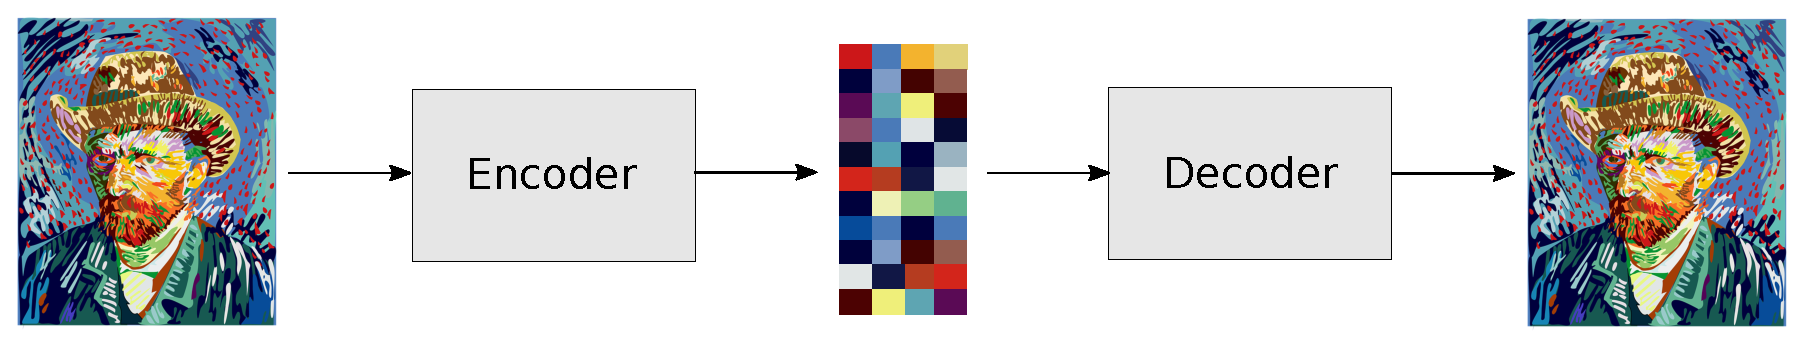
\includegraphics[scale=0.53]{background/autoencoder_black_box_architecture.eps}
\caption{A black-box description of an autoencoder. The autoencoder learns the identity function, and in turn, the encoder and decoder learn suitable encoding and decoding algorithms respectively.}
\label{fig:autoencoder_black_box_architecture}
\end{figure}

\subsection{Fully-Connected Autoencoders}

In dense feed-forward neural networks we may place a constraint on the latent space by reducing the number of neurons, as shown in Figure \ref{fig:autoencoder_architecture}. Images must be flattened into vectors to be fed as input. Consequently, any spatial information is destroyed in dense feed-forward neural networks.

\begin{figure}[h!]
\centering
\captionsetup{justification=centering}
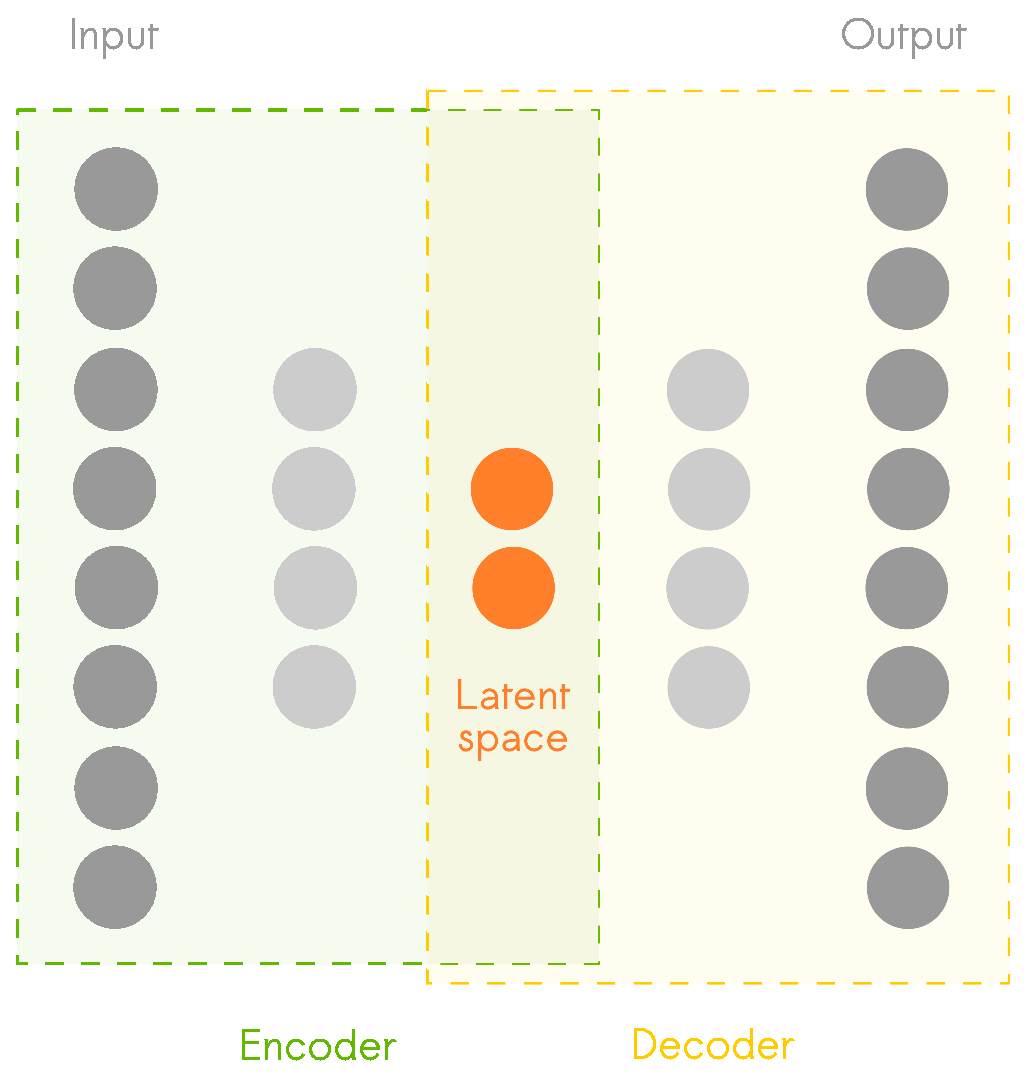
\includegraphics[scale=0.7]{background/autoencoder_architecture.eps}
\caption{The architecture of a fully-connected autoencoder. The latent space is constrained by having fewer neurons than the input and output layers.}
\label{fig:autoencoder_architecture}
\end{figure}

An example architecture is given in Table \ref{tab:fully_connected_autoencoder_architecture}, which was trained on MNIST images. Despite the severe restriction of $\sim96\%$ in the latent space, the network is capable of producing realistic reconstructions. For verification, a collection of samples from the dataset and their corresponding reconstructions are shown in Figure \ref{fig:fully_connected_autoencoder_mnist}.

\begin{table}[]
\centering
\captionsetup{justification=centering}
\label{tab:fully_connected_autoencoder_architecture}
\begin{tabular}{@{}ll@{}}
\toprule
\textbf{Module} & \textbf{Layers} \\ \midrule
Encoder & Dense (789) - Dense (32) \\
Decoder & Dense (32) - Dense (789) \\ \bottomrule
\end{tabular}
\caption{A simple fully-connected autoencoder with one hidden layer trained on MNIST. The Adam optimiser with learning rate $1e-4$ was used with a batch size of 1. After 15 epochs, the validation score was recorded to be $71.94$.}
\end{table}

\begin{figure}[h!]
\centering
\captionsetup{justification=centering}
\includegraphics[scale=0.95]{background/fully_connected_autoencoder_mnist.png}
\caption{A collection of images from the MNIST data set and their respective reconstructions using the fully-connected autoencoder specified in Table \ref{tab:fully_connected_autoencoder_architecture}. The original MNIST images are in odd columns, and their reconstructions to their immediate right.}
\label{fig:fully_connected_autoencoder_mnist}
\end{figure}

\subsection{Convolutional Autoencoders}

Convolutional layers have been shown to be effective in tasks with images as input \cite{Krizhevsky2012, Zeiler2014, Szegedy2015}. This is because spatial information is preserved in convolutional layers, and the number of trainable parameters is far less in a convolutional layer than it is in a fully connected layer.

When using convolutional layers, we may choose to use a dense latent space, or to keep the autoencoder fully-convolutional. In the former option, the spatial information is destroyed when flattening, which we will come to see is advantageous in the variational case.

\subsubsection{Dense Latent Space}

\subsubsection{Convolutional Latent Space}

\subsection{Variational Autoencoders}